\subsection{Comparative Peak Analysis of Simulation Results}

At the start of our different comparative analyses, we will first make a general rough analysis, creating a more simplified and easy-to-understand version of our results. As an example, in figure \ref{Fig:covid_info_graphs}, two histograms are visible, showcasing the only difference in the  simulation, namely the switching of contact tracing (CT). The two histograms display the occurrence of what the peak amount of infected is for a single day. So on the x-axis we have the peak amount of infected grouped together, and on y-axis we have the number of occurrences of the given grouped peak infected.

In the first histogram \ref{Subfig:covid_info_graphA}, the columns clearly show the effect of contact tracing. The maximum number of total infected within thousand drops of our simulation shows no higher than 210 infected of a total 12,500 population size, which equals to 1.68\% being infected of a total population. In other words, contact tracing seems to prove effective, since this is a very low total infection for the population. 

In the second histogram \ref{Subfig:covid_info_graphB}, the columns show a different reality. If COVID-19 were to run "invisibly", i.e. without society's knowledge and without the preventive measure of contact tracing, the simulation of a thousand drops estimates a maximum of 3857 infected. In comparison to histogram \ref{Subfig:covid_info_graphA}, in this simulation of thousand drops without contact tracing, the total infected population can reach as high as 30.8\% of the total population. 

\begin{figure}[H]
 \centering
  \begin{subfigure}{.45\textwidth}
    \centering
    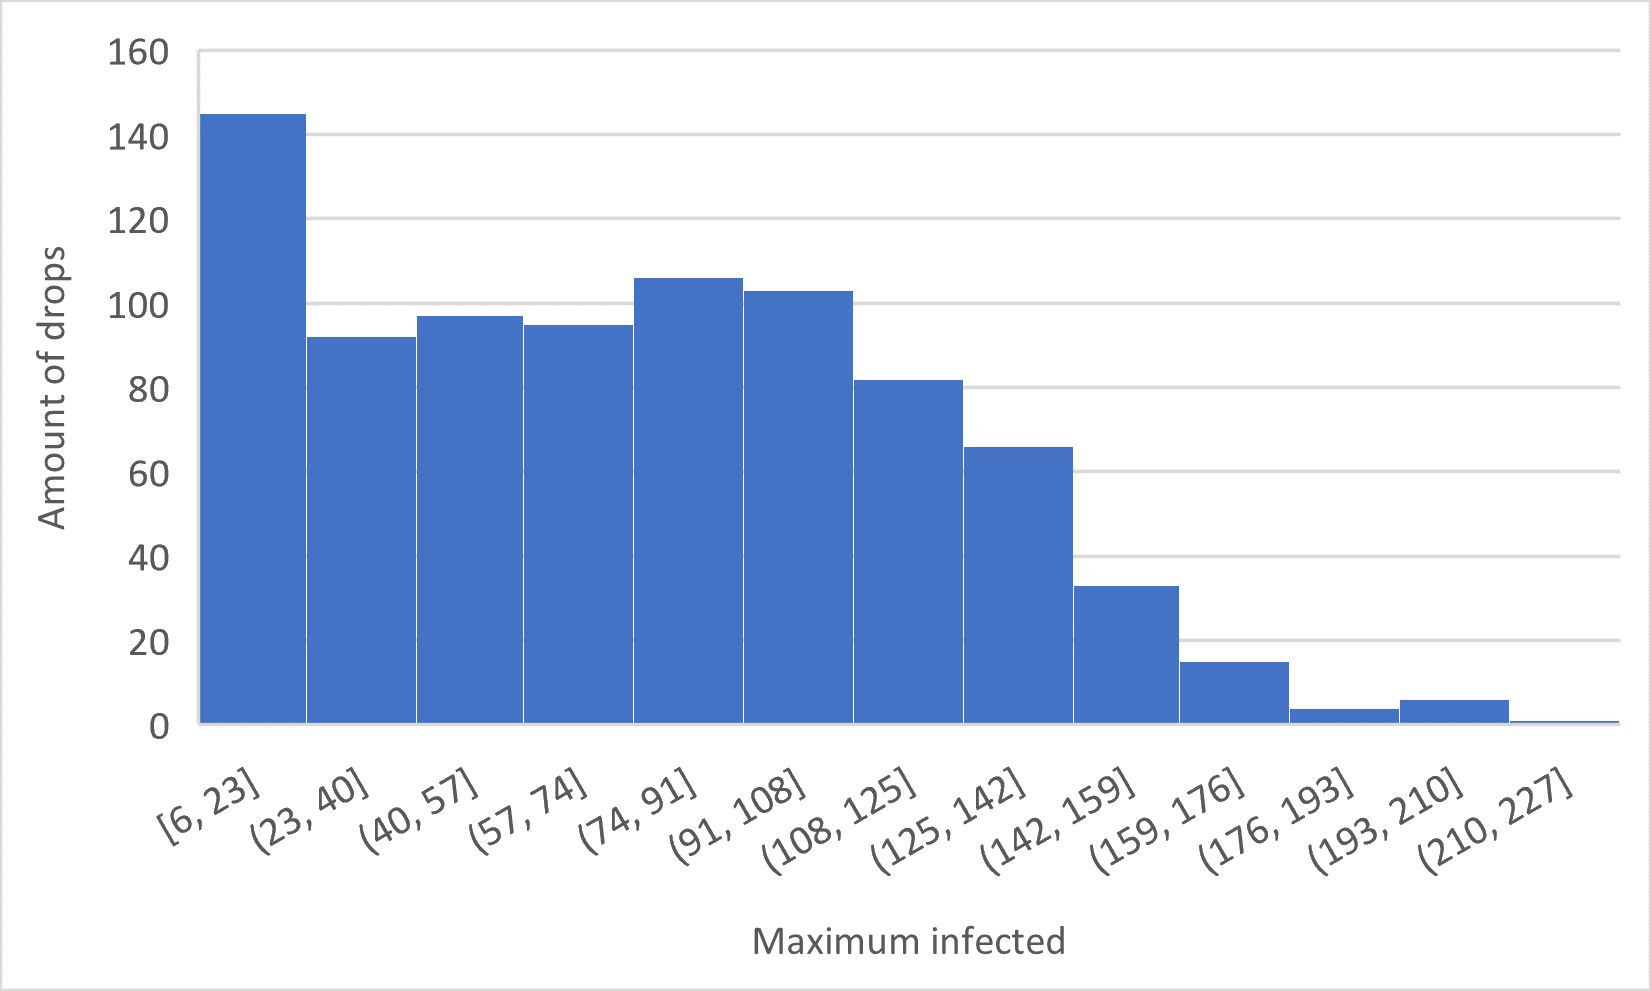
\includegraphics[width=.95\linewidth]{0_billeder/1k_ct_on_graph.png}
    \caption{With contact tracing}
    \label{Subfig:covid_info_graphA}
  \end{subfigure}
  \begin{subfigure}{.45\textwidth}
    \centering
    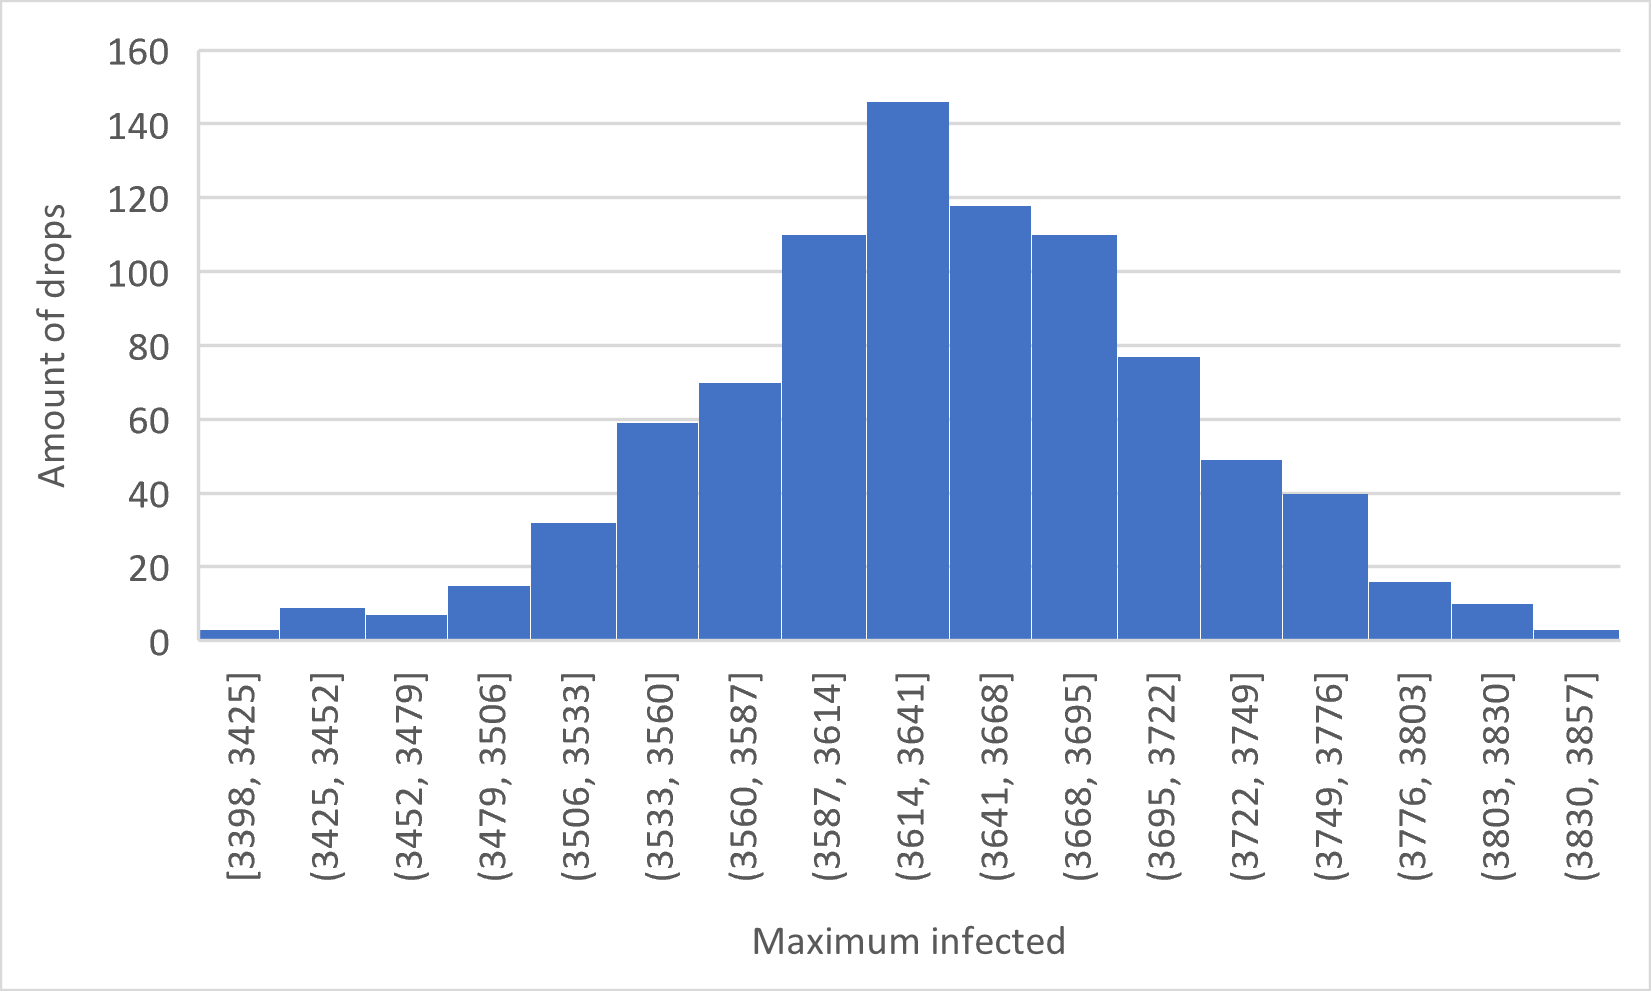
\includegraphics[width=.95\linewidth]{0_billeder/1k_ct_off_graph.png}
    \caption{Without contact tracing}
    \label{Subfig:covid_info_graphB}
  \end{subfigure} 
 \caption{Infection histograms with/without contact tracing.}
 \label{Fig:covid_info_graphs}
\end{figure}

Another way of documenting the effects of CT is comparing the amount of hospitalisations, which arguably is one of the worst case scenarios after infection. In this case, we once again compare data with two histograms, showcasing the maximum amount of hospitalisations on a simulation of 1000 drops, with/without contact tracing. 
A note here regarding the histograms is that the term "hospitalisation" covers from  to an intensive care bed with respirator, but we presume these hospitalisations are   

As a last remark, by roughly comparing the histograms, it is clear that contact tracing has an effect on spread of infection. To properly verify this conclusion, a sensitivity study must be made of the primary parameters, which the following section (\ref{sec: Sensitivity Study}).